\documentclass[12pt]{article}
\usepackage{amsthm}
\usepackage{amsmath}
\usepackage{array}
\usepackage{cancel}
\usepackage[thinc]{esdiff}
% \usepackage{gensymb}
\usepackage{geometry}
\usepackage{graphicx}
\usepackage{pgfplots}
\usepackage{siunitx}
\usepackage{wrapfig}
\usepackage{xcolor}

\title{Homework \#9, 4B}
\author{Donald Aingworth IV}
\date{March 19, 2025}

\pgfplotsset{width=8cm,compat=1.9}
\usepgfplotslibrary{external}
% \tikzexternalize

\renewcommand\thesubsection{\alph{subsection}}
\newcommand{\proj}{\text{proj}}
\newtheorem{theorem}{Theorem}

\begin{document}

\DeclareSIUnit{\mile}{mi}
\DeclareSIUnit{\gal}{gal}
\DeclareSIUnit{\foot}{ft}
\DeclareSIUnit{\hour}{h}
\DeclareSIUnit{\rad}{rad}
\DeclareSIUnit{\unit}{u}
\DeclareSIUnit{\dyne}{dyn}

\maketitle

\pagebreak
\section{Problem 2}
\begin{wrapfigure}{r}{0.25\textwidth}
    \vspace{-30pt}
    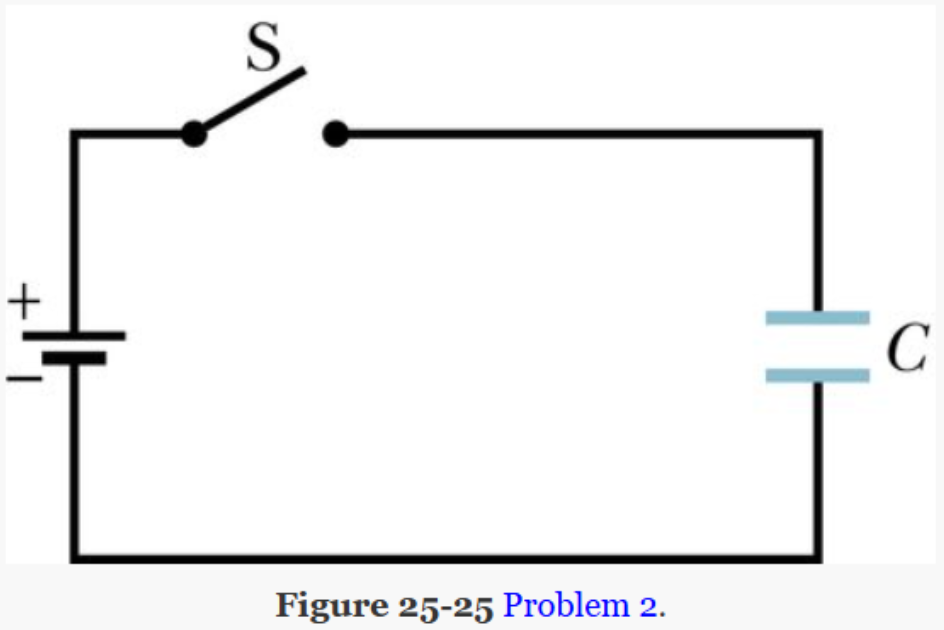
\includegraphics[width=0.25\textwidth]{picture_1.png} 
    % \label{fig:wrapfig}
\end{wrapfigure}
The capacitor in Fig. 25-25 has a capacitance of $25 \unit{\micro\farad}$ and is initially uncharged. 
The battery provides a potential difference of 120 V. 
After switch S is closed, how much charge will pass through it?

\subsection*{Solution: 3 mC}
We have an equation for this. 
For the capacitor to become fully charged, the charge that is the answer must pass into the capacitor and through the switch.
We have an equation for charge to enter a capacitor from voltage.
\begin{align*}
    q   &=  CV
        =   (25 \times 10^{-6}) * 120
        =   3000 \times 10^{-6} \unit{\coulomb}
        =   \boxed{\boxed{3 \unit{\milli\coulomb}}}
\end{align*}

\pagebreak
\section{Problem 4}
The plates of a spherical capacitor have radii 38.0 mm and 40.0 mm. 
(a) Calculate the capacitance. 
(b) What must be the plate area of a parallel-plate capacitor with the same plate separation and capacitance?

\subsection{Solution: 8.45 \texttimes\ 10$^{-11}$ F}
We have, from conference, the equation for the capacitance of a spherical capacitor.
We can use that to calculate the capacitance of our spherical capacitor.
\begin{align*}
    C   &=  4\pi\varepsilon_0 \frac{ab}{b - a}
        =   \frac{1}{8.99 \times 10^9} \frac{0.038 * 0.040}{0.040 - 0.038}\\
        &=  \frac{1}{8.99 \times 10^9} \frac{1.52 \times 10^{-3}}{2 \times 10^{-3}}
        =   \frac{0.76}{8.99 \times 10^9}\\
        &=  \boxed{8.45 \times 10^{-11} \unit{\farad}}
\end{align*}

\subsection{Solution: 191 cm$^2$}
The plate separation must be 2 \unit{\milli\meter} and the capacitance must be the above.
We have an equation that we can use for this.
\[
    C   =   \frac{\varepsilon_0 A}{d}
\]
\begin{align*}
    A   &=  \frac{Cd}{\varepsilon_0}
        =   \frac{8.45 \times 10^{-11} * 2 \times 10^{-3}}{8.85 \times 10^{-12}}\\
        &=  \frac{16.9}{8.85} \times 10^{-2} \unit{\meter^2}
        =   1.910 \times 10^{-2} \unit{\meter^2}\\
        &=  \boxed{191 \unit{\centi\meter^2}}
\end{align*}

\pagebreak
\section{Problem 5}
What is the capacitance of a drop that results when two mercury spheres, each of radius $R$ = 2.00 mm, merge?

\subsection*{Solution: 2.803 \texttimes\ 10$^{-13}$}
Mercury is a liquid at room temperature. 
The volume resultant would be equal to the volume of the two other spheres added together.
To avoid big numbers, we're just going to say that the small spheres will have radius $R$ and the big sphere will have radius $R'$. 
As such, we will find the value of $R'$.
\begin{gather*}
    V'  =   2V_0\\
    \frac{4}{3}\pi R'^3 =   2*\frac{4}{3}\pi R^3\\
    R'^3    =   2R^3\\
    R'      =   R\sqrt[3]{2}\\
    R'      =   0.002 * \sqrt[3]{2}
            =   2.520 \times 10^{-3} \unit{\meter}
\end{gather*}

From this, we can get the capacitance.
\begin{align*}
    C   &=  4\pi\varepsilon_0 R'
        =   \frac{2.520 \times 10^{-3}}{8.99 \times 10^9}
        =   \boxed{2.803 \times 10^{-13} \unit{\farad}}
\end{align*}

\pagebreak
\section{Problem 19}
% \begin{wrapfigure}{r}{0.4\textwidth}
%     \vspace{-30pt}
    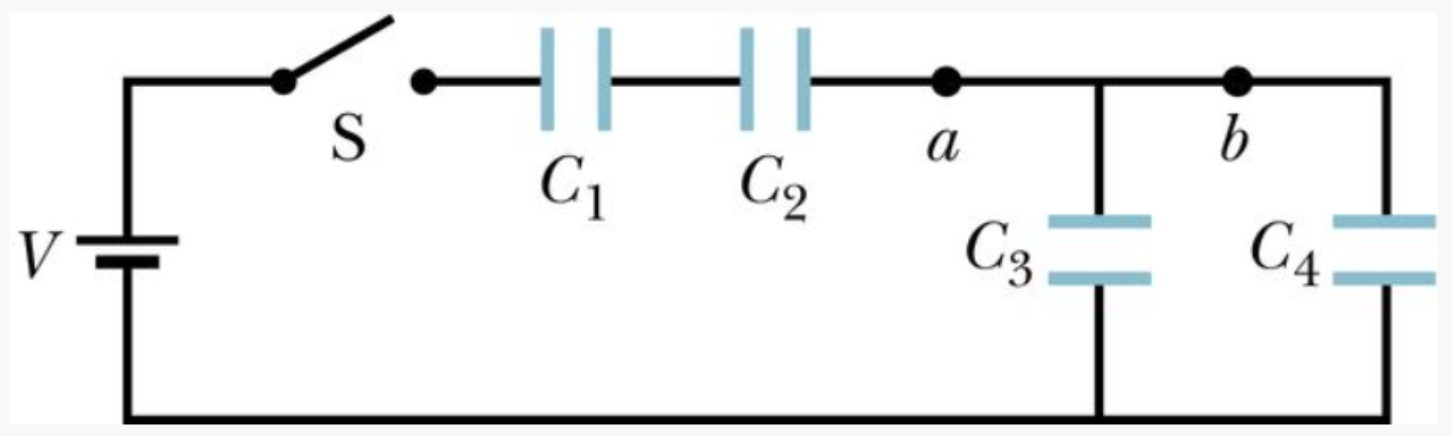
\includegraphics[width=\textwidth]{picture_4.png} 
%     % \label{fig:wrapfig}
% \end{wrapfigure}
In Fig. 25-34, the battery has potential difference $V = 9.0\unit{\volt}$, $C_2 = 3.0\unit{\micro\farad}$, $C_4 = 4.0\unit{\micro\farad}$, and all the capacitors are initially uncharged. 
When switch $S$ is closed, a total charge of $12 \unit{\micro\coulomb}$ passes through point $a$ and a total charge of $8.0 \unit{\micro\coulomb}$ passes through point $b$. 
What are (a) $C_1$ and (b) $C_3$?

\subsection{Solution: 4\textmu F}
Let's start by calculating $C_3$. 
Before the charge split, $12\unit{\micro\coulomb}$ of charge pass through the wire. 
It gets split, and $8\unit{\micro\coulomb}$ goes through the wire to $C_4$. 
The remaining $4\unit{\micro\coulomb}$ of charge has to go somewhere, so it goes through the wire to $C_3$.
Since electric potential difference is the same for each capacitor in parallel, we can create a formula for this.
\begin{align*}
    V_3 = V_4\\
    \frac{Q_3}{C_3} = \frac{Q_4}{C_4}\\
    \frac{C_3}{Q_3} = \frac{C_4}{Q_4}\\
    C_3 = \frac{Q_3}{Q_4}C_4
        &=  \frac{4}{8}*4 \unit{\micro\farad}
        =   \frac{4}{2} \unit{\micro\farad}
        =   2 \unit{\micro\farad}
\end{align*}

Now that we have $C_3$, we can use equivalence to find the capacitance of all capacitors together.
We know that the charge passing through any part of the circuit (not separated in parallel) is equal, and that charge must be $12\unit{\micro\coulomb}$.
We also know that the potential difference across the circuit must be the given potential difference of 9V. 
We can use this to calculate the capacitance across the circuit.
\[
    C_{\Sigma} = \frac{Q_0}{\Delta V} = \frac{12 \unit{\micro\coulomb}}{9 \unit{\volt}} = \frac{4}{3} \unit{\micro\farad}
\]

With this, we can set up a series of equations from capacitances in series and in parallel to find $C_1$.
\begin{align*}
    C_{34} = C_3 + C_4 &= 2 \unit{\micro\farad} + 4 \unit{\micro\farad} = 6 \unit{\micro\farad}\\
    \frac{1}{C_{\Sigma}} = \frac{1}{C_1} + \frac{1}{C_2} + \frac{1}{C_{34}}\\
    \frac{1}{C_1} = \frac{1}{C_{\Sigma}} - \frac{1}{C_1} - \frac{1}{C_2}
        &=  \frac{3}{4 \unit{\micro\farad}} - \frac{1}{3 \unit{\micro\farad}} - \frac{1}{6 \unit{\micro\farad}}
        =   \frac{9}{12 \unit{\micro\farad}} - \frac{4}{12 \unit{\micro\farad}} - \frac{2}{12 \unit{\micro\farad}}
        =   \frac{3}{12 \unit{\micro\farad}}\\
    C_1 &=  \boxed{4 \unit{\micro\farad}}
\end{align*}

\subsection{Solution: 2\textmu F}
We found it in part (a). It's \boxed{2\unit{\micro\farad}}.

\pagebreak
\section{Problem 22}
\begin{wrapfigure}{r}{0.4\textwidth}
    \vspace{-30pt}
    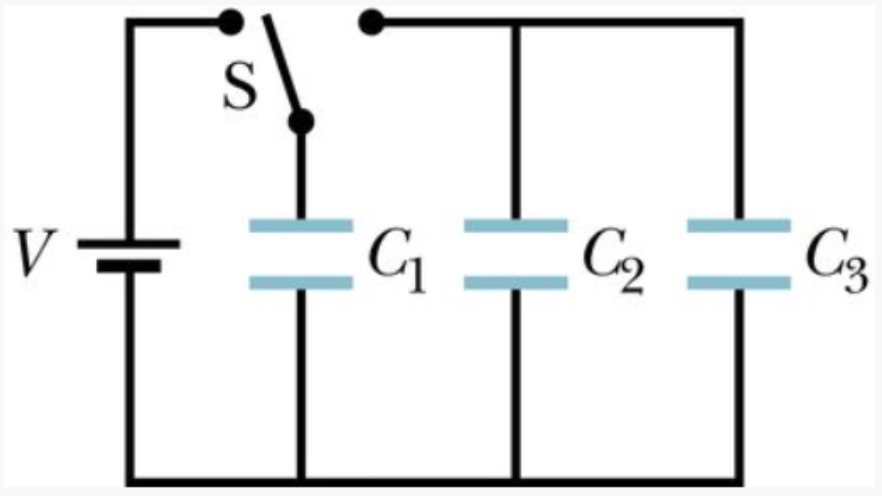
\includegraphics[width=0.4\textwidth]{picture_5.png} 
    % \label{fig:wrapfig}
\end{wrapfigure}
In Fig. 25-37, $V = 10 \unit{\volt}$, $C_1 = 10 \unit{\micro\farad}$, and $C_2 = C_3 = 20 \unit{\micro\farad}$. 
Switch S is first thrown to the left side until capacitor 1 reaches equilibrium. 
Then the switch is thrown to the right. 
When equilibrium is again reached, how much charge is on capacitor 1?

\subsection*{Solution: 20\textmu C}
Let's calculate the maximum charge on the capacitor $C_1$ , the charge it has when it gets released from the battery.
\begin{align*}
    Q   =   CV
        =   10\unit{\micro\farad}*10\unit{\volt}
        =   100\unit{\micro\coulomb}
\end{align*}

Now, when the capacitor is connected to the other two capacitors, it will have to share the capacitance with them.
For the sake of the problem, let's pretend that they are intead one capcitor, this time with charge $C_{23} = C_2 + C_3 = 40\unit{\micro\farad}$.
Since potential difference will be constant when we achieve equilibrium, we can have an equivalence here.
\begin{gather*}
    V_1 =   V_{23}\\
    Q   =   q_1 + q_{23} \rightarrow q_{23} = Q - q_{1}\\
    \frac{q_1}{C_1} =   \frac{q_{23}}{C_{23}}
        =   \frac{Q}{C_{23}} - \frac{q_1}{C_{23}}\\
    q_1 * \left( \frac{1}{C_1} + \frac{1}{C_{23}} \right)   =   \frac{Q}{C_{23}}\\
    q_1 =   \frac{Q}{C_{23}}*\left( \frac{1}{C_1} + \frac{1}{C_{23}} \right)^{-1}
\end{gather*}
\begin{align*}
    q_1 &=  \frac{100\unit{\micro\coulomb}}{40\unit{\micro\farad}}*\left( \frac{1}{10\unit{\micro\farad}} + \frac{1}{40\unit{\micro\farad}} \right)^{-1}\\
        &=  \frac{100\unit{\micro\coulomb}}{40\unit{\micro\farad}} * \frac{40\unit{\micro\farad}}{5}\\
        &=  \boxed{20\unit{\micro\coulomb}}
\end{align*}
This fits well with an idea that charge is given proportionally to the capacitance compared to the total capacitance, but that's a story for another day.

\pagebreak
\section*{Charge Proportionality Theorem}
That day is today. Let's define and prove a proportionality theorem for the charge that passes through parallel capacitors.
We'll call it the Parallel Capacitor Equivalent Charge Proportionality Theorem, or PCECPT for short.
\begin{theorem}[PCECPT]
    Let $C$ be a perfect capacitor or equivalent to a perfect capacitor unique in its parallel line through part of a circuit made up on only perfect wires.
    The charge from the power source that will go to $C$ compared to the total charge traveling through all the parallel wires is equivalent to the capacitance of $C$ compared to the total capacitance of all capacitors in parallel.
\end{theorem}
\begin{proof}
    Let C have a capacitance $C_1$.
    Suppose that there are a nonzero number $n$ of capacitors in parallel. 
    We can express the equivalent capacitance of all capacitors in parallel as $C_{eq}$ and do the same for a generic equivalent capacitor in parallel $C_i$.
    We can replace this with values of charge, with $Q_{eq}$ being the combined charge of all capacitors and $Q_i$ being the charge passing through one equivalent parallel capacitor.
    \begin{gather*}
        Q_{eq} = \frac{C_{eq}}{V}   \Leftrightarrow V = \frac{C_{eq}}{Q_{eq}}\\
        Q_i =   \frac{C_i}{V}       \Leftrightarrow V = \frac{C_i}{Q_i}
    \end{gather*}

    Since the electric potential difference is always the same in parallel capacitors, we can use the reflexive property and then substitute in values.
    From that, we can get the ratio we're looking for.
    \begin{gather*}
        V   =   V\\
        \frac{C_{eq}}{Q_{eq}}   =   \frac{C_i}{Q_i}\\
        \frac{Q_{eq}}{C_{eq}}   =   \frac{Q_i}{C_i}\\
        \frac{Q_i}{C_i}         =   \frac{Q_{eq}}{C_{eq}}\\
        Q_i =   \frac{C_i}{C_{eq}}Q_{eq}
    \end{gather*}
    This gives us what we're looking for. QED.
\end{proof}

\pagebreak
\section{Problem 23}
\begin{wrapfigure}{r}{0.4\textwidth}
    \vspace{-30pt}
    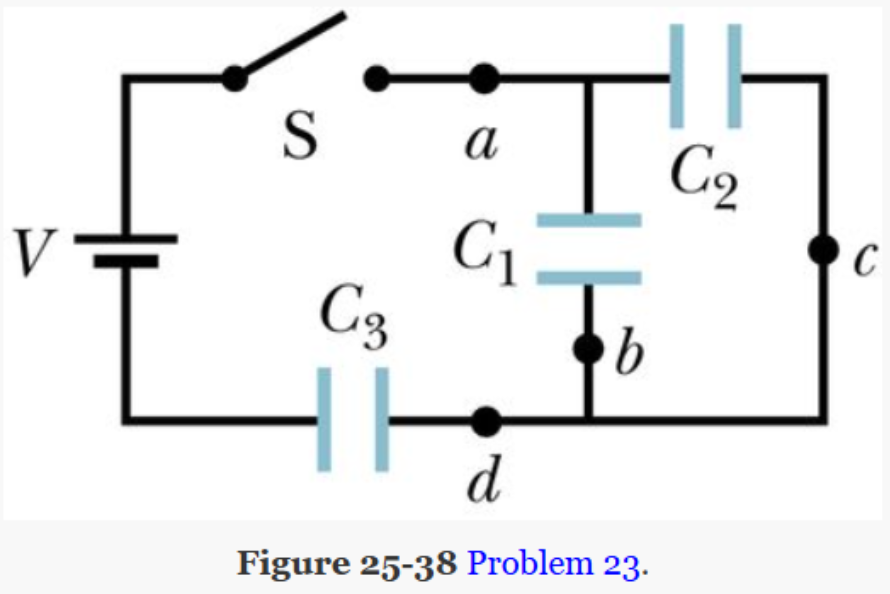
\includegraphics[width=0.4\textwidth]{picture_6.png} 
    % \label{fig:wrapfig}
\end{wrapfigure}
The capacitors in Fig. 25-38 are initially uncharged. 
The capacitances are $C_1 = 4.0 \unit{\micro\farad}$, $C_2 = 8.0 \unit{\micro\farad}$, and $C_3 = 12 \unit{\micro\farad}$, and the battery's potential difference is $V = 12 \unit{\volt}$. 
When switch S is closed, how many electrons travel through (a) point a, (b) point b, (c) point c, and (d) point d? 
In the figure, do the electrons travel up or down through (e) point b and (f) point c?

\subsection{Solution: 4.49\texttimes 10$^{14}$}
Let's make an equivalent capacitor. 
\begin{align*}
    C_{12}  &=  C_1 + C_2 = 4 + 8 = 12 \unit{\micro\farad}\\
    C_{123} &=  \left( \frac{1}{C_{12}} + \frac{1}{C_3} \right)^{-1}
        =   \left( \frac{1}{12} + \frac{1}{12} \right)^{-1}
        =   \left( \frac{2}{12} \right)^{-1}
        =   \frac{12}{2}
        =   6\unit{\micro\farad}
\end{align*}

We can apply our favorite equation to this.
\begin{align*}
    q   &=  CV
        =   6 \times 10^{-6} * 12
        =   72 \times 10^{-6} \unit{\coulomb}
\end{align*}

Dividing this by the charge of an electron would give us the number of electrons crossing. 
\begin{equation}
    \frac{q}{e} = \frac{72 \times 10^{-6}}{1.602 \times 10^{-19}}
        =   \boxed{4.49 \times 10^{14}}
\end{equation}

\subsection{Solution: 1.50\texttimes 10$^{14}$}
The charge that goes through each parallel line on the circuit will be proportional to the total capacitance of each individual line's equivalent capacitor.
In this instance, the capacitance of point $b$'s line is $4\unit{\micro\farad}$ compared to the total $12\unit{\micro\farad}$. 
We can apply this fraction to the charge. 
\[\frac{4}{12}*72 = \boxed{1.50 \times 10^{14}}\]

\subsection{Solution: 3.00\texttimes 10$^{14}$}
We know that 24\textmu C of the 72\textmu C went to the line with point (b).
The remaining 48\textmu C has to go somewhere, and its only space it can go to is the line with point (c).
As such, the answer is the 48\textmu C divided by the charge of an electron, so \boxed{3.00 \times 10^{14}}.

\subsection{Solution: 4.49\texttimes 10$^{14}$}
In series, the charge passing through any given point is the same. 
As such our answer would be the same as in part (a), or \boxed{4.49 \times 10^{14}}.

\subsection{Solution: up}
Electrons travel from the negative plate to the positive plate. 
Looking at the closest capacitor ($C_1$), the negative plate is the one closer to the negative part of the battery, so that would be the bottom one.
As such, it would travel from the bottom to the top, otherwise known as \underline{up}.

\subsection{Solution: up}
Electrons travel from the negative plate to the positive plate. 
Looking at the closest capacitor ($C_2$) and moving it slightly towards the negative side of the battery without changing the core structure of the circuit, the negative plate is the one closer to the negative part of the battery, so that would be the bottom one.
As such, it would travel from the bottom to the top, otherwise known as \underline{up}.

\pagebreak
\section{Problem 31}
A $2.0 \unit{\micro\farad}$ capacitor and a $4.0 \unit{\micro\farad}$ capacitor are connected in parallel across a 300 V potential difference.
Calculate the total energy stored in the capacitors.

\subsection*{Solution: 0.27J}
These capacitors have a collective capacitance of 6\unit{\micro\farad}. 
We have a formula for total energy stored in a capacitor, which can be applied to the equivalent to find the energy equivalent to the total energy contained in these two capacitors collectively.
\begin{align*}
    U   &=  \frac{1}{2}CV^2
        =   \frac{1}{2}*(6 \times 10^{-6})*300^2
        =   3 * 9 \times 10^{-2}
        =   \boxed{0.27 \unit{\joule}}
\end{align*}

\pagebreak
\section{Problem 32}
A parallel-plate air-filled capacitor having area $40\unit{\centi\meter^2}$ and plate spacing $1.0 \unit{\milli\meter}$ is charged to a potential difference of $600 \unit{\volt}$. 
Find (a) the capacitance, (b) the magnitude of the charge on each plate, (c) the stored energy, (d) the electric field between the plates, and (e) the energy density between the plates.

\subsection{Solution: 3.5419pF}
The dielectric constant of air is $\kappa = 1.00054$.
This is a parallel plate capacitor, so we have a simple formula for the capacitance. 
\begin{align*}
    C   &=  \frac{\kappa\varepsilon_0 A}{d}
        =   \frac{1.00054*(8.85 \times 10^{-12})*(40 \times 10^{-4})}{10^{-3}}\\
        &=  1.00054 * 8.85 * 40 \times 10^{-13}
        =   \boxed{35.419 \unit{\pico\farad}}
\end{align*}

\subsection{Solution: 21.251nC}
We'll use the formula for the charge stored. 
\begin{align*}
    q   &=  CV
        =   35.419 \times 10^{-12} * 600
        =   21.251 \times 10^{-9} \unit{\coulomb}
        =   \boxed{21.251 \unit{\nano\coulomb}}
\end{align*}

\subsection{Solution: 6.375\textmu J}
\begin{align*}
    U   &=  \frac{q^2}{2C}
        =   \frac{(21.251 \times 10^{-9})^2}{2*35.419 \times 10^{-12}}
        =   \frac{4.516 \times 10^{-16}}{70.838 \times 10^{-12}}
        =   \boxed{6.375 \times 10^{-6} \unit{\joule}}
\end{align*}

\subsection{Solution: 6\texttimes 10$^5$N/C}
\begin{align*}
    V   &=  Ed \rightarrow
    E   =   \frac{V}{d}
        =   \frac{600}{10^{-3}}
        =   \boxed{6 \times 10^5 \unit{\newton/\coulomb}}
\end{align*}

\subsection{Solution: 1.5938 J/m$^3$}
\begin{align*}
    u   &=  \frac{1}{2}\kappa\varepsilon_0 E^2
        =   \frac{1}{2}1.00054*(8.85 \times 10^{-12})*(6 \times 10^5)^2
        =   8.85 * 18 \times 10^{-2}\\
        &=  159.38 \times 10^{-2}
        =   \boxed{1.5938 \unit{\joule/\meter^3}}
\end{align*}

\pagebreak
\section{Problem 35}
Assume that a stationary electron is a point of charge. 
What is the energy density $u$ of its electric field at radial distances (a) $r = 1.00 \unit{\milli\meter}$, (b) $r = 1.00 \unit{\micro\meter}$, (c) $r = 1.00 \unit{\nano\meter}$, and (d) $r = 1.00 \unit{\pico\meter}$? 
(e) What is $u$ in the limit as $r \rightarrow 0$?

\subsection{Solution: 9.1782\texttimes 10$^{-18}$ J/m$^3$}
We have a formula for the energy density.
\begin{gather*}
    u = \frac{1}{2}\varepsilon_0E^2\\
    E   =   \frac{kq}{r^2}
\end{gather*}\begin{align*}
    u   &=  \frac{\varepsilon_0}{2}*\frac{k^2q^2}{r^4}
        =   \frac{8.85 \times 10^{-12}}{2}*\frac{(8.99 \times 10^9)^2*(-1.602 \times 10^{-19})^2}{(10^{-3})^4}\\
        &=  \frac{8.85 * 8.99^2 * 1.602^2}{2} \times \frac{10^{-12} * 10^{18} * 10^{-38}}{10^{-12}}\\
        &=  \frac{8.85*80.8201*2.566404}{2} \times 10^{-20}
        =   917.82 \times 10^{-20}\\
        &=  \boxed{9.1782 \times 10^{-18} \unit{\joule/\meter^3}}
\end{align*}

\subsection{Solution: 9.1782\texttimes 10$^{-6}$ J/m$^3$}
Let's imagine the formula we has as a fraction, composed on $r^4$ on the bottom and some constant $c$ on the top. 
We know that since only the radius changes, all other components stay the same, so $c$ is constant.
We can acknowledge that $u_a$ (our answer to part (a)) is equal to $\frac{c}{r_a^4}$.
Comparing radii, we can know that $r_b = r_a \times 10^{-3}$.
\begin{align*}
    u_b &=  \frac{c}{r_b^4}
        =   \frac{c}{(r_a \times 10^{-3})^4}
        =   \frac{c}{r_a} \times 10^{12}\\
        &=  9.1782 \times 10^{-18} \times 10^{12}\\
        &=  \boxed{9.1782 \times 10^{-6} \unit{\joule/\meter^3}}
\end{align*}

\subsection{Solution: 9.1782\texttimes 10$^{6}$ J/m$^3$}
We'll just do the same thing. 
Comparing radii, we can know that $r_c = r_a \times 10^{-6}$.
\begin{align*}
    u_c &=  \frac{c}{r_c^4}
        =   \frac{c}{(r_a \times 10^{-6})^4}
        =   \frac{c}{r_a} \times 10^{24}\\
        &=  9.1782 \times 10^{-18} \times 10^{24}\\
        &=  \boxed{9.1782 \times 10^{6} \unit{\joule/\meter^3}}
\end{align*}

\subsection{Solution: 9.1782\texttimes 10$^{18}$ J/m$^3$}
We'll just do the same thing. 
Comparing radii, we can know that $r_c = r_a \times 10^{-9}$.
\begin{align*}
    u_d &=  \frac{c}{r_d^4}
        =   \frac{c}{(r_a \times 10^{-9})^4}
        =   \frac{c}{r_a} \times 10^{36}\\
        &=  9.1782 \times 10^{-18} \times 10^{36}\\
        &=  \boxed{9.1782 \times 10^{18} \unit{\joule/\meter^3}}
\end{align*}

\subsection{Solution: $\infty$}
We can take a limit.
\begin{align*}
    u   &=  \underset{r\to 0}{\lim}\left( \frac{\varepsilon_0}{2}*\frac{k^2q^2}{r^4} \right)
        =   \frac{\varepsilon_0k^2q^2}{2}*\underset{r\to 0}{\lim}\left( \frac{1}{r^4} \right)\\
        &=  \frac{\varepsilon_0k^2q^2}{2}*\infty
        =   \boxed{\infty}
\end{align*}

\pagebreak
\section{Problem 47}
A certain substance has a dielectric constant of $2.8$ and a dielectric strength of $18 \unit{\mega\volt/\meter}$. 
If it is used as the dielectric material in a parallel-plate capacitor, what minimum area should the plates of the capacitor have to obtain a capacitance of $7.0 \times 10^{-2} \unit{\micro\farad}$ and to ensure that the capacitor will be able to withstand a potential difference of $4.0 \unit{\kilo\volt}$?

\subsection*{Solution: 6277 cm$^2$}
The potential difference has to be $V = 4.0 \unit{\kilo\volt}$ and the capacitance has to be $C = 70 \unit{\nano\farad}$. 
We have a couple formulas for use in this. 
We have the formula for Gauss' Law with a dialectric ($\varepsilon_0 \oint\kappa\vec{E}\cdot\,dA = q$), the formula for capacitance and charge ($q = CV$), and the formula for the capacitance of a parallel plate capacitor ($C = \frac{\varepsilon_0 A}{d}$). 
Since the electric potential difference will be constant throughout the capacitor, the potential difference of the capacitor can be written as $\Delta V = E \Delta x$, which can be turned into, for the instance of the capacitor, $V = Ed$.
We can use three of these formulas as a basis to get a formula with exclusively known values.
\begin{gather*}
    V = Ed \Leftrightarrow C = \frac{\varepsilon_0 A}{d}\\
    d   =   \frac{V}{E}\\
    C   =   \frac{\varepsilon_0 A E}{V}
\end{gather*}

We should not forget to turn use dielectric constant with the permativity of free space.
Then, we can solve for the area.
\begin{align*}
    &C  =   \frac{\kappa\varepsilon_0 AE}{V}\\
    A   &=  \frac{CV}{\kappa\varepsilon_0 E}
        =   \frac{(70 \unit{\nano\farad})*(4.0 \unit{\kilo\volt})}{(2.8)(8.85 \times 10^{-12})(18 \unit{\mega\volt})}\\
        &=  \frac{70*4}{2.8*8.85*18} * \frac{10^{-9}*10^3}{10^{-12}*10^6}\unit{\meter^2}\\
        &=  \frac{280}{446.04} \unit{\meter^2}
        =   0.6277 \unit{\meter^2}
        =   \boxed{6277\unit{\centi\meter^2}}
\end{align*}
\end{document}